%\documentclass[a4paper,12pt]{article}
\documentclass[a4paper,10pt,twocolumn]{article}
%\usepackage[brazil]{babel}
%\usepackage{amsmath}
\usepackage{graphicx}
\bibliographystyle{plain} 

\begin{document}

  \title{A Solution of the General Model for a Digital System }
  \author{
    Filipi Damasceno Vianna\\
    \small{Pontifical Catholic University of Rio Grande do Sul}\\
    \small{E-mail: \texttt{filipi@em.pucrs.br}}
    \footnote{Correspondence should be addressed to this autor at: 
    Pontificia Universidade Catolica do Rio Grande do Sul, Mechanical
    and Mecatronics Engineering Dept. Av. Ipiranga, 6681. Predio 
    30/Bloco 7. CEP 90619-900.  Porto Alegre-RS. Brazil. Phone:
    55-51-3320-3584. Fax: 55-51-3320-3625.}
  \and
    Daniel Fink\\
    \small{Pontifical Catholic University of Rio Grande do Sul}\\
    \small{E-mail: \texttt{dfink@crt.net.br}}
  \and
    Jos{\'e} In{\'a}cio Coelho\\
    \small{University of Rio dos Sinos Valey}\\
    \small{E-mail: \texttt{jic@aquila.com.br}}
}
	
  \date{Porto Alegre, May, 1998.}
  \maketitle

  \section{Introdution}

    \hspace{.5 cm}
    The intent of this research is presents the Logical \textbf{Es{\c c}{\~a}o(n~m~p)}
    in its 3rd year of investigation. The Logical \textbf{Es{\c c}{\~a}o(n~m~p)} goes
    towards the 5th generations computers, vanishing the called \textit{Von 
    Neumann�s Bottleneck} from the current computers. Enable, also, a
    deterministic  perception of the variable inputs and working in 
    real time. From its datas, the theoretical aspects of this new
    computing system was investigated and tried to use it in lots of systems to
    confirm its functioning and evaluate the advantages against the
    conventional controllers.

    The significance of this work is the contribution for a search to eliminate
    the Von Neumann bottleneck from the present computational architecture. It
    deals by putting in practice the ``General Model for a Digital System'',
    (PHISTER, 1958)\cite{phister}, that has a entire random functioning and
    processing in real time. In abridgment, the right control system.

    The Von Neumann bottleneck is a present computer characteristic where the
    information is obliged to pass by a centralized stage which will deal,
    arrange and decide the destiny that the program flow must to take.

    % Cite Vector computers lik PowerPC G4 and supercomputers as
    % another try to eliminate the Von Neumann's bottleneck

    In other way the advanced technology, like computers architecture and
    computing language project, use very elevated math abstractions. To
    become this knowledge accessible to market and mainly towards technical
    terms, specially to Technical High Schools, is the fulfillment of this
    work.

  \section{How it does work}

    \hspace{.5 cm}
    Following the theories developed in the thesis published in the book 
    ``Es{\c c}{\~a}o (\textit{n}~\textit{m}~\textit{p}) - A Non Von 
    Neumann Computer'', from the teacher W. W. Martins\cite{escao}, the 
    \textbf{Es{\c c}{\~a}o} is a sequential machine that use a lot of devices from 
    the family \textbf{ROM} (read only memory), who can works in
    asynchronous mode, without clock, keeping out the use of the traditional
    flip-flop devices, or even synchronism using one of the inputs as a
    temporal step, which is gonna be called of $X\oslash$, who is input
    undependable variable.

    It has then two kinds of machines, being the first one of asynchronous
    functioning, with 100\% inner capacity occupied to memorize the programs
    and conversions in a real time. We got $2^n$ synchronism combinations
    possible in the inputs, being in the number of undependable variables,
    or monitored sensors for example.

    The second kind would be an \textbf{Es{\c c}{\~a}o} functioning with a temporal
    step in low frequency. It means we are gonna use a independent variable
    as a clock input and then we are gonna have 50\% of inner memory capacity
    utilization to save the programs. So we have $2^n - 1$ possible
    combination to a variation of the other independent variables. It is good
    to remember that the functioning continues in a real time and with
    intelligence of searching among the programs the suitable outputs to the
    aleatoric occurrences of the inputs.

    \begin{center}
      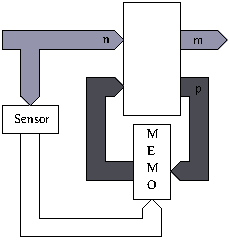
\includegraphics[width = 6.5 cm, height = 6.5 cm]{logo.pdf}
    \end{center}

    \begin{itemize}     

      \item \textit{n} number of \textbf{independents} Boolean variables
            (input)

      \item \textit{m} number of \textbf{dependable} Boolean variables
            (output)

      \item \textit{p} number of \textbf{internal} Boolean variables
            (feedback or memories)

    \end{itemize}

    So then, a \textbf{Es{\c c}{\~a}o} (n-m-p) is nothing more than a computacional
    machine, that using the microelectronic devices (Integration in a Very
    Large Scale) like RAM, ROM, EPROM, etc., creates a control able to
    eliminate completely a microprocessor, having economical advantages in
    ``real time''.

    It is good to remember that comparing both structures, it got a great
    technology advantage, which is the whole elimination of the
    microprocessor, who takes together the historical ``virus''  of the
    Von Neumann Bottleneck.

    Another characteristic of a \textbf{Es{\c c}{\~a}o} machine is the
    non-probabilistic behaviour. It means that it do not have a segment
    period of time to verify the input events, but we have a kind of entire
    monitoring of the independent variables, which give us a great fidelity
    towards the perception information received.


    \subsection{Understanding Es{\c c}{\~a}o (n-m-p)}

      \hspace{.5 cm}
      To really understand the functioning of a \textbf{Es{\c c}{\~a}o} is important
      to know two concepts.

      \begin{itemize}

        \item \textsf{\textbf{EIE}} Stable Internal State

        \item \textsf{\textbf{EII}} Instable Internal State

      \end{itemize}


      To explain this topics, let is go back to Phister Theory, in the title
      \textit{``Logical Design of Digital Computers''} 1958\cite{phister},
      who tries to solve the \textit{``General Model for a Digital System''}

      With the intention to give a particular nomenclature to \textbf{Es{\c c}{\~a}o}
      logic, the name of the variables used by Phister to explain the
      \textit{``General Model for a Digital System''}, (p, r, y) was changed
      by (n,m,p) as follows below:

      \begin{itemize}     

        \item \textit{n} number of \textbf{independents} Boolean variables
              (input)

        \item \textit{m} number of \textbf{dependable} Boolean variables
              (output)

        \item \textit{p} number of \textbf{internal} Boolean variables
              (feedback or memories)

      \end{itemize}

      The last number [ \textbf{p} ] deals towards the system of the memory,
      who can be computed by the base-two, giving the \textsf{\textbf{EIE}}
      number. These will define the space to store of sequential programs
      that the machine will execute.

      $$2^p = EIE$$

      Any similar from a Phister Model towards the logic shown here is not
      mere coincidence. This work, among several things, suggests a solution
      to the \textit{``General Model for a Digital System''} using the VLSI
      technology.

      The amount of \textsf{\textbf{EIE}} will define the space to store the
      sequential programs that the machine will execute. So, for a
      \textbf{Es{\c c}{\~a}o} machine, as a \textsf{\textbf{EIE}} is simply a memory
      space, or else, a BYTE. As each byte uses one address, and to access
      must be gived the right address in the inputs of memory device.

      Remembering about input variables, it always will be in the EPROM�s
      address bus, sharing place with the feedback variables. It means that
      each input change shows a new address. And from there starts a process
      of \textbf{Es{\c c}{\~a}o} machine!


      \begin{enumerate}

        \item The EPROM found itself in a Stable Internal State (
              \textsf{\textbf{EIE}}), a constant input,  and the feedback is
              identical as in the input as in the output. This state can be
              called of standby, because it is waiting a new order.

        \begin{center}
          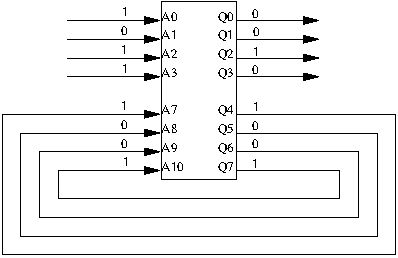
\includegraphics[width = 7 cm, height = 5 cm]{passo1.pdf}
        \end{center}

        \item Happens a variation in the inputs.

        \begin{center}
          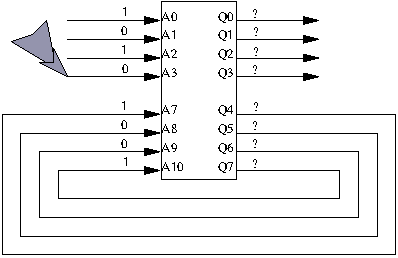
\includegraphics[width = 7 cm, height = 5 cm]{passo2.pdf}
        \end{center}

        \item The EPROM gets it as a new address and immediately sends a
              new content in the output.

        \begin{center}
          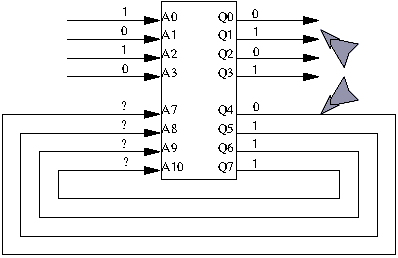
\includegraphics[width = 7 cm, height = 5 cm]{passo3.pdf}
        \end{center}


        \item Now there is a Instable Internal State (\textsf{\textbf{EII}}),
              where through the feedback lines, a part from new data goes
              back to the adress bus, pointing out a new address. It is good
              to remember that this process is extremely fast, having the
              speed from the changing electrons in silicon.

        \begin{center}
          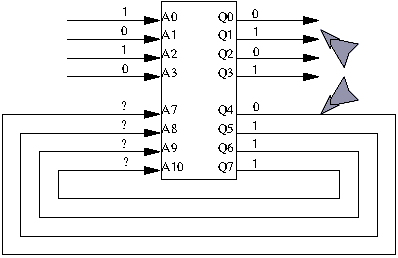
\includegraphics[width = 7 cm, height = 5 cm]{passo3.pdf}
        \end{center}

        \item The new adress pointed out by feedback will be again Stable
              Internal State [\textsf{\textbf{EIE}}]. It has the exact
              information that was requested with the change in the input
              bit. This answer stays still in the EPROM output, who stays
              again in standby, waiting for the new order.

        \begin{center}
          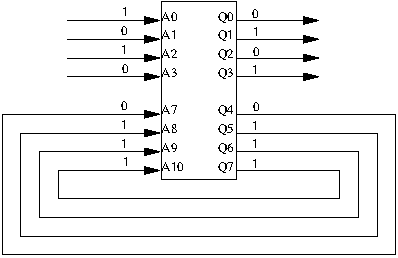
\includegraphics[width = 7 cm, height = 5 cm]{passo4.pdf}
        \end{center}

        \item Note that the new address pointed out by \textsf{\textbf{EII}}
              must have, in the bits reserved to feedback, the same data of
              the anterior adress. So, the \textsf{\textbf{EIE}} store the 
              answers that are needed and that the machine should give
              according  to input variables. What determines the content
              of \textsf{\textbf{EIE}} is the programmer. In another words
              the \textsf{\textbf{DDD}} is made uniquely
              \textsf{\textbf{EIE}}.

      \end{enumerate}

      On the order side, the \textsf{\textbf{EII}} are not
      determined by the programmer, but by the software that is
      gonna generate the FIRMWARE. It is function is to direct
      the correct addressing to EPROM. Another function of a
      \textsf{\textbf{EII}} is to make a suggestion of output
      to be availed by another circuit, that will accept or 
      not(see A/D Converter). So we have several
      \textsf{\textbf{EII}} to a \textsf{\textbf{EIE}}, despite
      of usually the proportion is one by one.


      \subsection{The Es{\c c}{\~a}o(\textit{n~m~p}) Machine Conception}

        \hspace{.5 cm}
        To project a sequential machine being synchronous or asynchronous,
        using the logic \textbf{Es{\c c}{\~a}o}, I got a follow methodology. The
        steps below were used as a foundation to the accomplishments of
        the prototypes for the practical presentation of this research.

        \begin{enumerate}

          \item Accomplish a list of internal stable state
                \textsf{\textbf{EIE}}
          \item Elect the independent variable (input VAB), the dependent
                variables (output VAB) and the internal variables (feedback
                VAB), drawing in a operational block, the logic circuit
                sequential switch, whose project have been intended.
          \item Drawing of the correspondent GRAPH with or without the
                temporal step (variable $X\oslash$), depending on the
                application.
          \item The $X\oslash$ introduction as temporal step, will, allow
                that the \textsf{\textbf{EIE}} list, gave lately change to
                ``project matrix'' where will be introduced the unstable
                state concepts and stable state.
          \item It�s possible optionally, to transform the ``project
                matrix'' in a kind of truth-table equivalent.
          \item By the numerical definition, that will be seen later, 
                from the Project Matrix or the equivalent truth table,
                we�ll get a expression of FABs (Booleans Arithmetic
                Functions) that will correspond to the direct programming
                of the own technologic device VLSI, who can be any unit of
                the family RAM / ROM / EPROM  / EEPROM and so on.

        \end{enumerate}

        Now let�s go for a bigger zoom in the \textbf{Es{\c c}{\~a}o} diagram, as
        shown in the picture below. 

        \begin{center}
          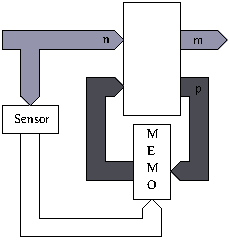
\includegraphics[width = 5 cm, height = 5 cm]{logo.pdf}
        \end{center}

        Here is the ROM  device (Reading Only Memory). The MEMOS are the
        feedback memories ($Y_{1},...,Y_{P}$) that is gonna determine the
        internal state tables \textsf{\textbf{EIE}} of the controllers.
        Here is the general condition to an EPROM:

        $$n^{o} EIE = 2^{p}$$

        The Aleatoric Changes Detector is the memory�s feedback trigger,
        for every variation in the input variables: X1,...,Xn

        In general conditions to an EPROM 2716 (2k Bytes) we have
        following:

        $$n + p \leq 11$$

        Address bus is made by 11 bits that takes the $2_{11}$ memory
        addresses.

        $$n + p \leq 8 \bullet N$$

        The number of unused exits plus the feedback variable are
        always less or equal to 8, which is the induced limitation
        made by the memory of the Data Bus. It is possible to increase
        the numbers adding more memory devices in the circuit. Then
        it has N $\bullet$ 8 outputs, where N is the amount of 2716,
        or another memory device.

  \bibliography{escao_works}
\end{document}
